% Clase del documento
\documentclass[12pt, letterpaper]{article}

% Definicion del preambulo
% Para insertar imágenes
\usepackage{graphicx}

% Para tener referencias
\usepackage{hyperref}

% Para poner matemáticas
\usepackage{amsthm, amssymb}

% Comentarios en pdf
\setlength {\marginparwidth }{2cm}
\usepackage{todonotes}

% Matrices
\usepackage{amsmath}

% Para poner definiciones con color
\usepackage[most]{tcolorbox}

% Colores
\usepackage{xcolor}

% Quita sangrías/Pone saltos en párrafos
%\usepackage{parskip}

% Español
\usepackage[spanish]{babel}

% imagenes svg
\usepackage{svg}

% para insertar imágenes en una posición estricta
\usepackage{float}

% Definición personalizada de tcolorbox
\newtcolorbox{miDefinicion}[2][]{
  colback=teal!5!white,
  colframe=teal!75!black,
  coltitle=white,
  fonttitle=\bfseries,
  title=Definición: #2,
  arc=2mm,
  boxrule=0.8pt,
  enhanced,
  drop shadow,
  #1
}


% Para poner call outs chidos
\usepackage{mdframed}
% Definimos el estilo del callout con línea a la izquierda
\newmdenv[
  topline=false,      % Quita la línea superior
  bottomline=false,   % Quita la línea inferior
  rightline=false,    % Quita la línea derecha
  leftline=true,      % Activa solo la línea izquierda
  linecolor=cyan,     % Color de la línea (puedes usar blue, red, etc.)
  linewidth=3pt,      % Grosor de la línea
  innerleftmargin=10pt, % Espacio entre la línea y el texto
  innerrightmargin=0pt,
  innertopmargin=0pt,
  innerbottommargin=0pt
]{miencuadre}

\usepackage{booktabs}

\usepackage{dirtree}

\usepackage{varwidth}

\usepackage{fancyvrb}

\usepackage{pmboxdraw}
\DeclareUnicodeCharacter{251C}{\textSFviii} % ├
\DeclareUnicodeCharacter{2500}{\textSFx}    % ─
\DeclareUnicodeCharacter{2514}{\textSFii}   % └
\DeclareUnicodeCharacter{2502}{\textSFxi}   % │

% Titulo, autor y fecha
\title{\textbf{\textcolor{blue}{ROS}}}
\author{Ricardo Victoria}
\date{octubre 2027}

% Inicio del documento
\begin{document}

% Insertamos el preambulo
\maketitle

\section{Espacio de trabajo y Paquetes}
\subsection{Estructura General}
Cuando utilizamos ROS 2, debemos organizar nuestras carpetas y archivos de una forma muy específica. De manera muy general, la organización va así: 

\textbf{espacio de trabajo}\textgreater\textbf{paquetes}\textgreater\textbf{nodos de ros}. 
\vspace{0.8em}

Un espacio de trabajo es una carpeta que contiene todas las carpetas y archivos de nuestro proyecto. Un paquete es una carpeta que contiene los nodos que programemos. Un nodo es un archivo de código fuente, usualmente un objeto.

Más detalladamente, la estructura de un espacio de trabajo de ros se ve así:

\vspace{1em}

\begin{center}
\begin{minipage}{1.1\textwidth}
\dirtree{%
.1 \textbf{ros2\_ws/} \dotfill Espacio de trabajo (\textit{Workspace}).
.2 \textbf{src/} \dotfill Directorio raíz del código fuente.
.3 \textbf{mi\_paquete\_cpp/} \dotfill Paquete de C++ (\textit{ament\_cmake}).
.4 CMakeLists.txt \dotfill Instrucciones de compilación de CMake.
.4 package.xml \dotfill Declaración de dependencias y metadatos.
.4 include/ \dotfill Archivos de cabecera (.hpp).
.4 src/ \dotfill Código fuente ejecutable.
.5 \textbf{nodo\_cpp.cpp} \dotfill Nodo escrito en C++.
.3 \textbf{mi\_paquete\_py/} \dotfill Paquete de Python (\textit{ament\_python}).
.4 package.xml \dotfill Declaración de dependencias y metadatos.
.4 setup.py \dotfill Configuración de instalación de Python.
.4 setup.cfg \dotfill Definición de ejecutables/puntos de entrada.
.4 mi\_paquete\_py/ \dotfill Módulo principal de Python.
.5 \textbf{nodo\_py.py} \dotfill Nodo escrito en Python.
.2 \textbf{build/} \dotfill Archivos intermedios (generado por \texttt{colcon}).
.2 \textbf{install/} \dotfill Puntos de entrada y binarios (generado por \texttt{colcon}).
.2 \textbf{log/} \dotfill Registros de depuración (generado por \texttt{colcon}).
}
\end{minipage}
\end{center}

\vspace{1.5em}

En el diagrama anterior, se muestra la estructura de un espacio de trabajo de ROS, con dos paquetes, uno de C++ y otro de Python.

\subsection{Creación de un Espacio de Trabajo}
Vamos a crear un espacio de trabajo en la terminal de Linux. Primero, creamos una carpeta que será el espacio de trabajo, a esta carpeta la nombraremos \texttt{taller\_ws} (nótese que \texttt{ws} viene de workspace o espacio de trabajo). Entonces creamos la carpeta con \texttt{mkdir taller\_ws}. 

\begin{verbatim}
usuario@equipo:~/ROS$ mkdir taller_ws
\end{verbatim}

Luego, dentro del espacio de trabajo crearemos una carpeta llamada \texttt{src} (esa carpeta por convensión se llama así).

\begin{verbatim}
usuario@equipo:~/ROS$ cd taller_ws
usuario@equipo:~/ROS/taller_ws$ mkdir src
\end{verbatim}

Dentro de \texttt{src}, vamos a hacer un paquete de C++ llamado \texttt{viz\_package\_cpp}. Queremos que este paquete contenga:

\begin{itemize}
    \item un archivo \texttt{CMakeLists.txt}
    \item una carpeta \texttt{include/}
    \item una licencia Apache 2.0
    \item un archivo \texttt{package.xml}
    \item una carpeta con un nodo \texttt{src/viz\_node.cpp} 
\end{itemize}

Lo anterior lo podemos hacer con el siguiente comando:

\begin{verbatim}
ros2 pkg create --build-type ament_cmake --node-name \
viz_node viz_package_cpp --license Apache-2.0
\end{verbatim}

\begin{center}
  \begin{Verbatim}[gobble=4]
    usuario@equipo:~/ROS/taller_ws$ cd src
    usuario@equipo:~/ROS/taller_ws/src$ ros2 pkg create --build-type ament_cmake \
    --node-name viz_node viz_package_cpp --license Apache-2.0
  \end{Verbatim}
\end{center}

\begin{figure}[H] 
  \centering    
  \makebox[\textwidth][c]{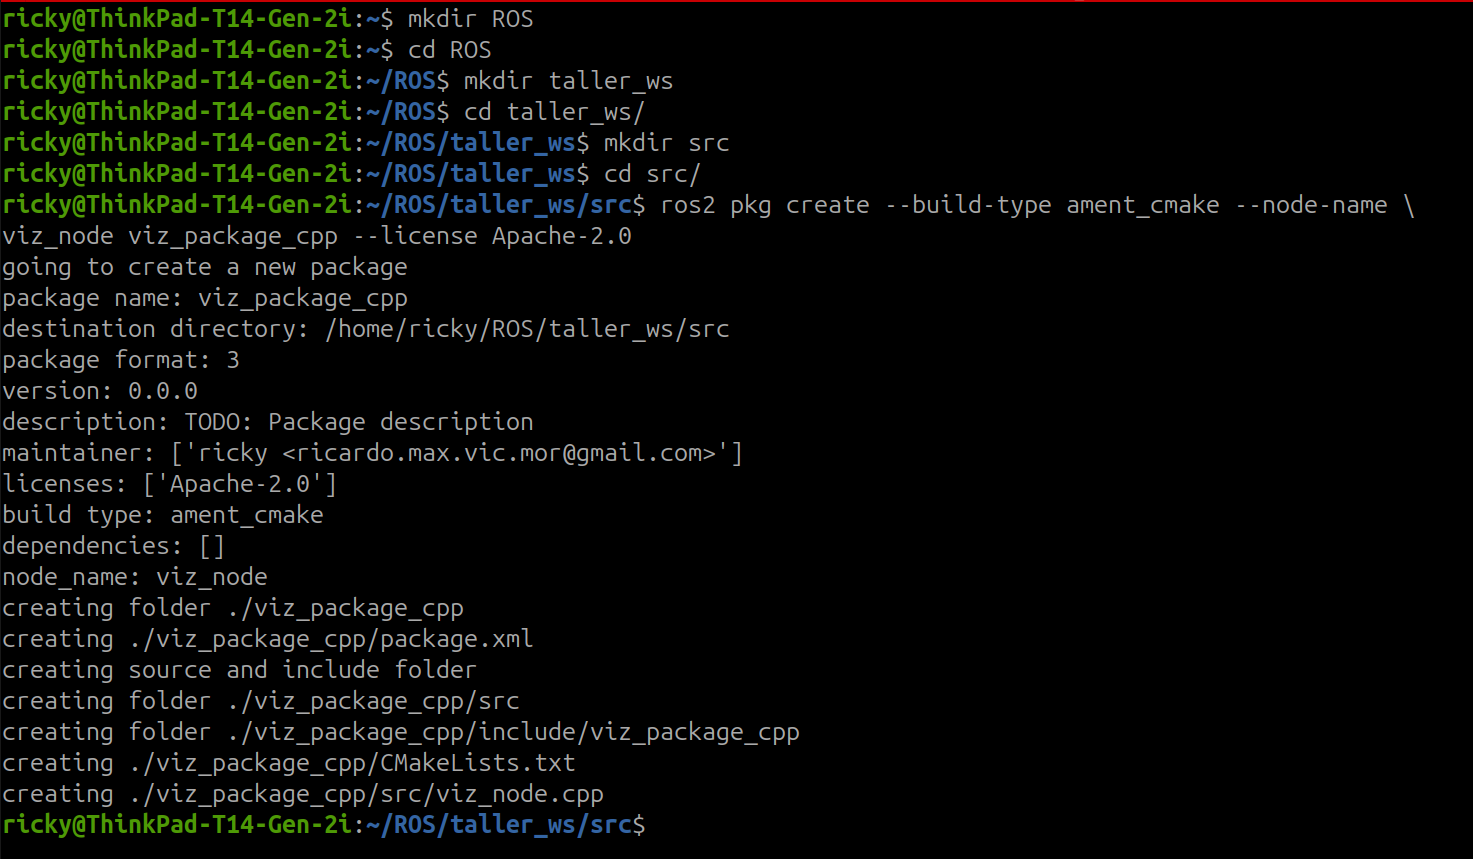
\includegraphics[width=1.4\textwidth]{imagenes/1.png}}
  \caption{Creación de Espacio de Trabajo, y Paquete con Nodo.}
  \label{fig:mi_imagen}
\end{figure}

A continuación se muestra cómo quedó la estructura del paquete.

\begin{center}
  \begin{Verbatim}[gobble=4]
    usuario@equipo:~/ROS/taller_ws/src$ tree
    .
    └── viz_package_cpp
        ├── CMakeLists.txt
        ├── include
        │   └── viz_package_cpp
        ├── LICENSE
        ├── package.xml
        └── src
            └── viz_node.cpp

    5 directories, 4 files
  \end{Verbatim}
\end{center}

\begin{figure}[H] 
  \centering    
  \makebox[\textwidth][c]{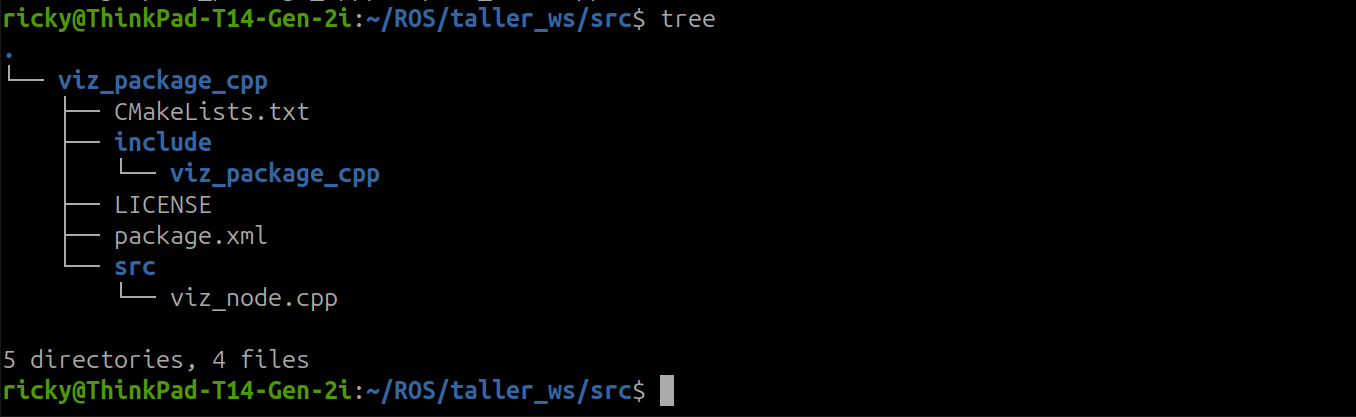
\includegraphics[width=1.4\textwidth]{imagenes/1-2.png}}
  \caption{Estructura del Paquete.}
  \label{fig:mi_imagen}
\end{figure}

[en otras iteraciones, explicaré el contenido de los archivos anteriores].

\subsection{Compilar y Ejecutar}
Una vez que tenemos la estructura que definimos anteriormente. Procedemos a compilar el espacio de trabajo, y ejecutar el nodo que creamos. El nodo que creamos anteriormente sólo devuelve un hola mundo. 

Para compilar, usamos \texttt{colcon}, la herramienta de compilación por línea de comandos oficial de ROS 2. Su función es orquestar la construcción de múltiples paquetes dentro de un espacio de trabajo.

Podemos compilar e instalar todo el espacio de trabajo con:

\begin{center}
  \begin{Verbatim}[gobble=4]
    colcon build
  \end{Verbatim}
\end{center}

o podemos compilar e instalar un paquete específico con:

\begin{center}
  \begin{Verbatim}[gobble=4]
    colcon build --packages-select <nombre del paquete>
  \end{Verbatim}
\end{center}

\begin{figure}[H] 
  \centering    
  \makebox[\textwidth][c]{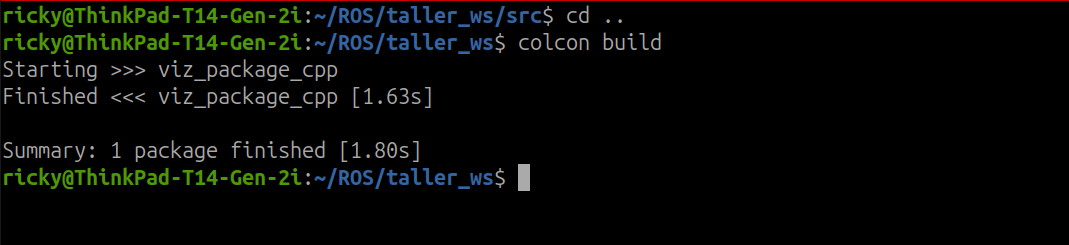
\includegraphics[width=1.4\textwidth]{imagenes/2.png}}
  \caption{Compilación.}
  \label{fig:mi_imagen}
\end{figure}

Luego, para ejecutar un nodo de un paquete, abrimos una nueva terminal (no se debe ejecutar en la misma terminal donde se compiló, porque puede fallar la ejecución), y en la nueva terminal activamos el overlay con:
\begin{center}
  \begin{Verbatim}[gobble=4]
    source install/local_setup.bash
  \end{Verbatim}
\end{center}
y ejecutamos el nodo con:
\begin{center}
  \begin{Verbatim}[gobble=4]
    ros2 run <nombre del paquete> <nombre del nodo>
  \end{Verbatim}
\end{center}

\begin{figure}[H] 
  \centering    
  \makebox[\textwidth][c]{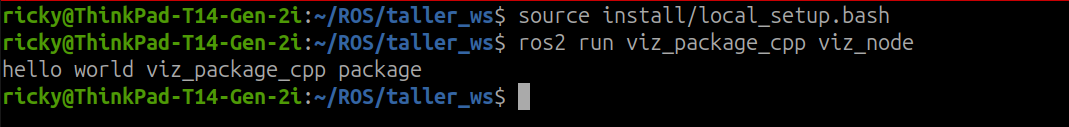
\includegraphics[width=1.4\textwidth]{imagenes/2-2.png}}
  \caption{Ejecución del Nodo.}
  \label{fig:mi_imagen}
\end{figure}

\section{Archivos de Lanzamiento}
Anteriormente vimos cómo ejecutar un nodo. Pero en un proyecto grande de ROS, necesitaremos lanzar muchos más nodos. Necesitamos una forma de ejecutar muchos nodos con un sólo comando. Para esos sirven los archivos de lanzamiento o launch files. 

Un launch file permite realizar varias configuraciones para el ambiente y ejecutar multiples nodos.

Para poder usar launch files, realizar los siguientes pasos:
\begin{enumerate}
    \item Dentro del archivo \texttt{package.xml} del paquete, agregar la siguiente línea dentro de las etiquetas \texttt{<package>}:
    
\begin{center}
  \begin{Verbatim}[gobble=4]
    <exec_depend> ros2launch </exec_depend>
  \end{Verbatim}
\end{center}

\begin{figure}[H] 
  \centering    
  \makebox[\textwidth][c]{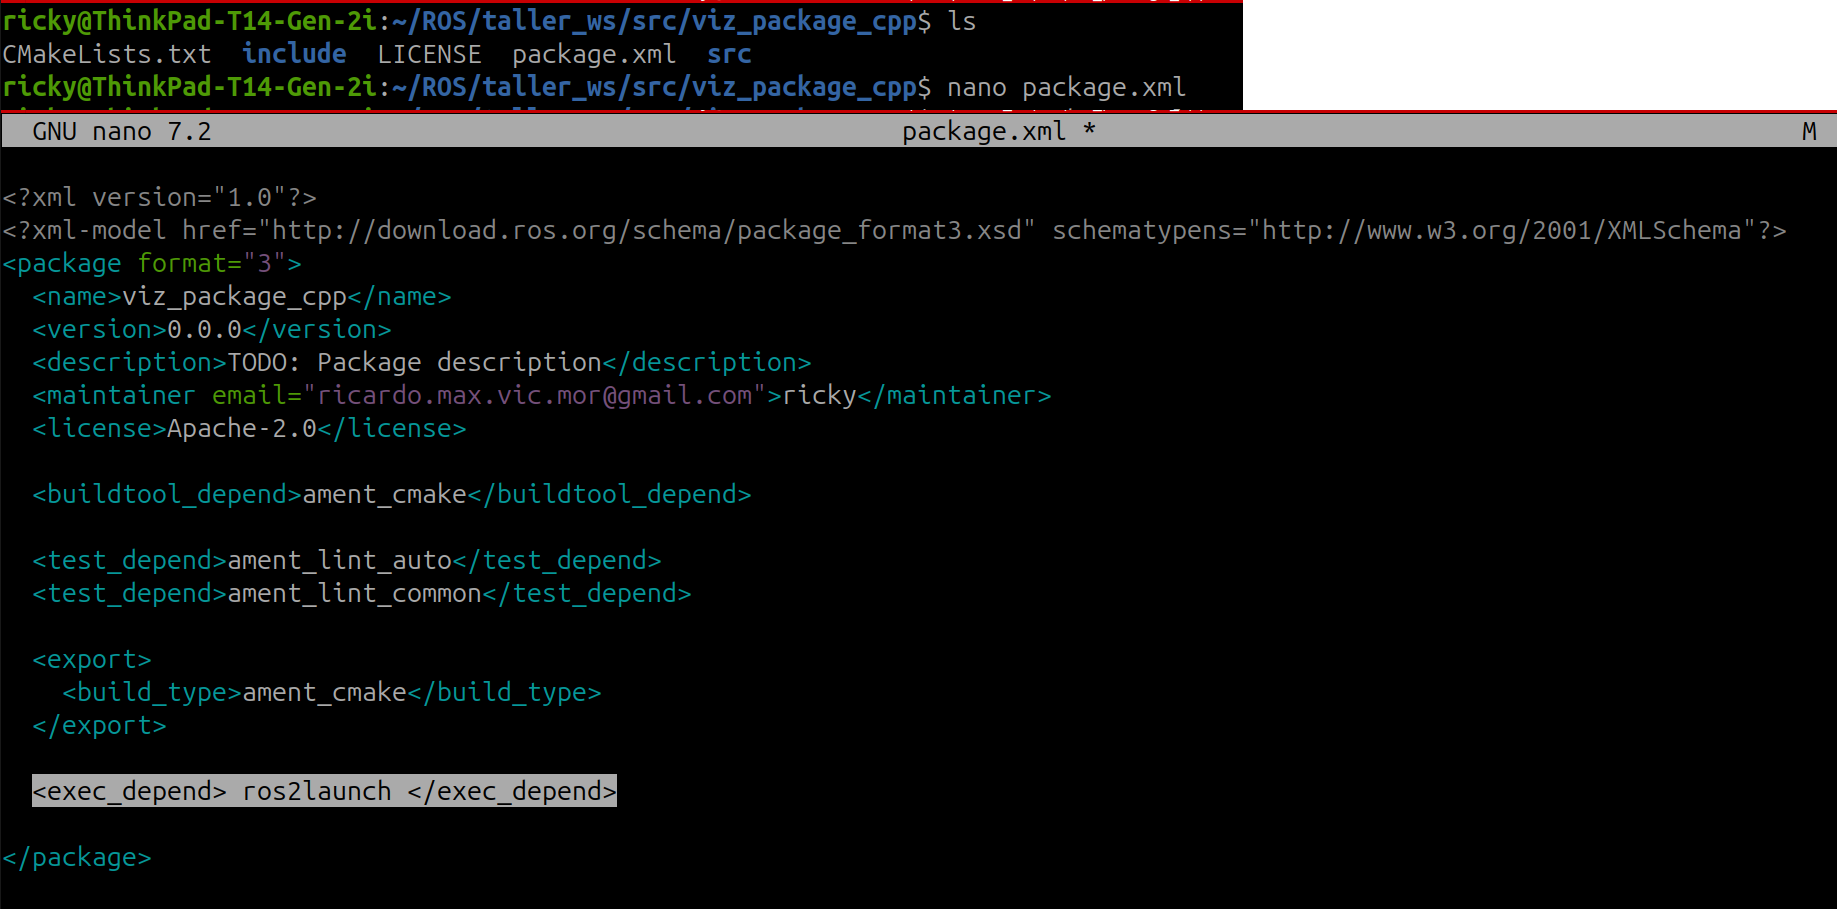
\includegraphics[width=1.4\textwidth]{imagenes/package.png}}
  \caption{Edición de package.xml para habilitar launch files.}
  \label{fig:mi_imagen}
\end{figure}

\item Crear una carpeta \texttt{launch} dentro del paquete.

\begin{figure}[H] 
  \centering    
  \makebox[\textwidth][c]{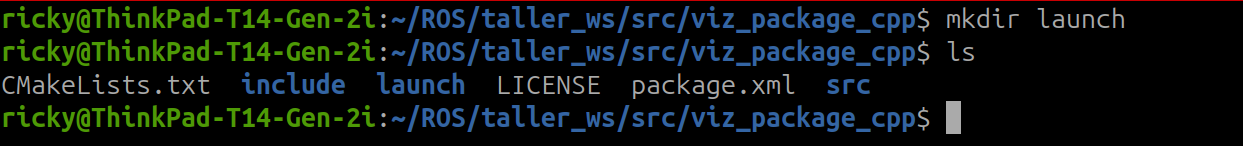
\includegraphics[width=1.4\textwidth]{imagenes/4.png}}
  \caption{Creación carpeta launch.}
  \label{fig:mi_imagen}
\end{figure}

\item Dentro de la carpeta \texttt{launch}, creamos un archivo de lanzamiento\\\texttt{viz\_launch.py} con el contenido que se ve en la imagen siguiente.

\begin{figure}[H] 
    \centering    
    \makebox[\textwidth][c]{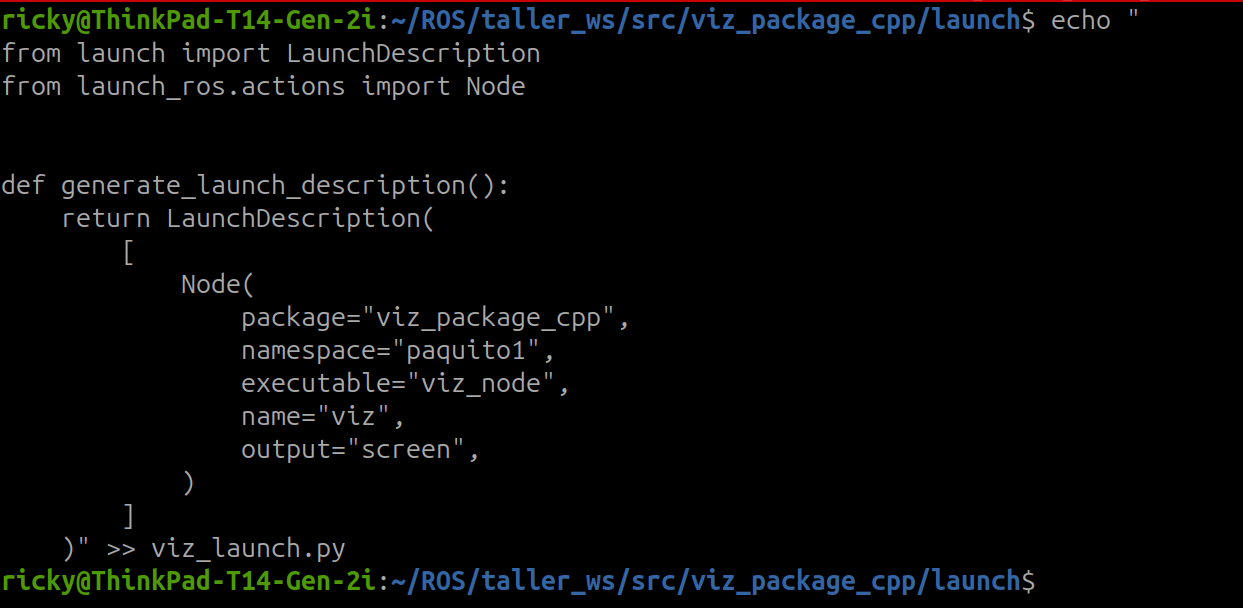
\includegraphics[width=1.4\textwidth]{imagenes/vizlaunch.png}}
    \caption{Creación carpeta launch.}
    \label{fig:mi_imagen}
\end{figure}
\item Volvemos a compilar.
\end{enumerate}




Con los pasos anteriores, ya podemos hacer uso de nuestro archivo de lanzamiento \texttt{viz\_launch.py}, el cual lanza el nodo \texttt{viz\_node}. Para lanzar el launch file nos ubicamos en la carpeta \texttt{launch} del paquete, y hacemos:

\begin{center}
  \begin{Verbatim}[gobble=4]
    ros2 launch <nombre archivo lanzamiento>
\end{Verbatim}
\end{center}

\begin{figure}[H] 
    \centering    
    \makebox[\textwidth][c]{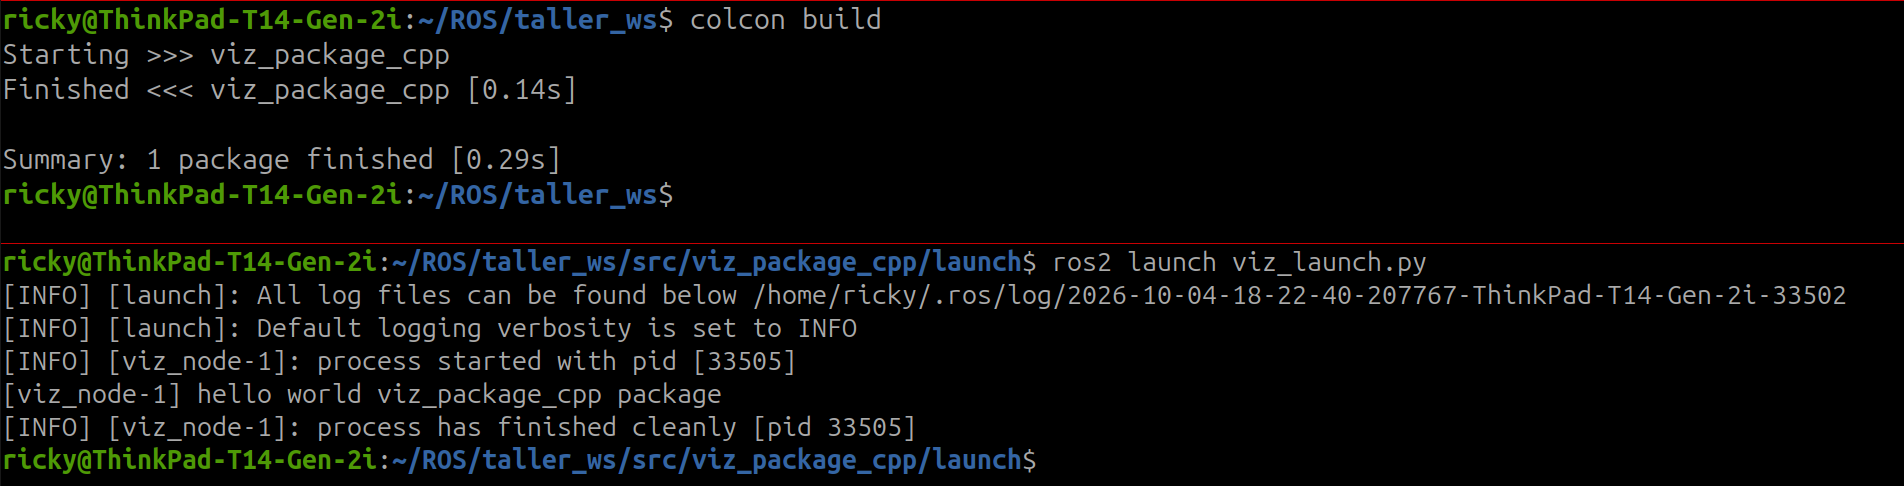
\includegraphics[width=1.4\textwidth]{imagenes/lanzandomix.png}}
    \caption{Lanzando nuestro primer launch file.}
    \label{fig:mi_imagen}
\end{figure}


Ahora, para poder lanzar el launch file sin tener que ubicarnos en la carpeta launch, hacemos lo siguiente:
\begin{enumerate}
  \item Abrir el archivo \texttt{CMakeLists.txt} del paquete, y agregar lo siguiente:
  \begin{center}
    \begin{Verbatim}[gobble=4]
      install(DIRECTORY
      launch
      DESTINATION share/${PROJECT_NAME}
      )
    \end{Verbatim}
  \end{center}

  \begin{figure}[H] 
      \centering    
      \makebox[\textwidth][c]{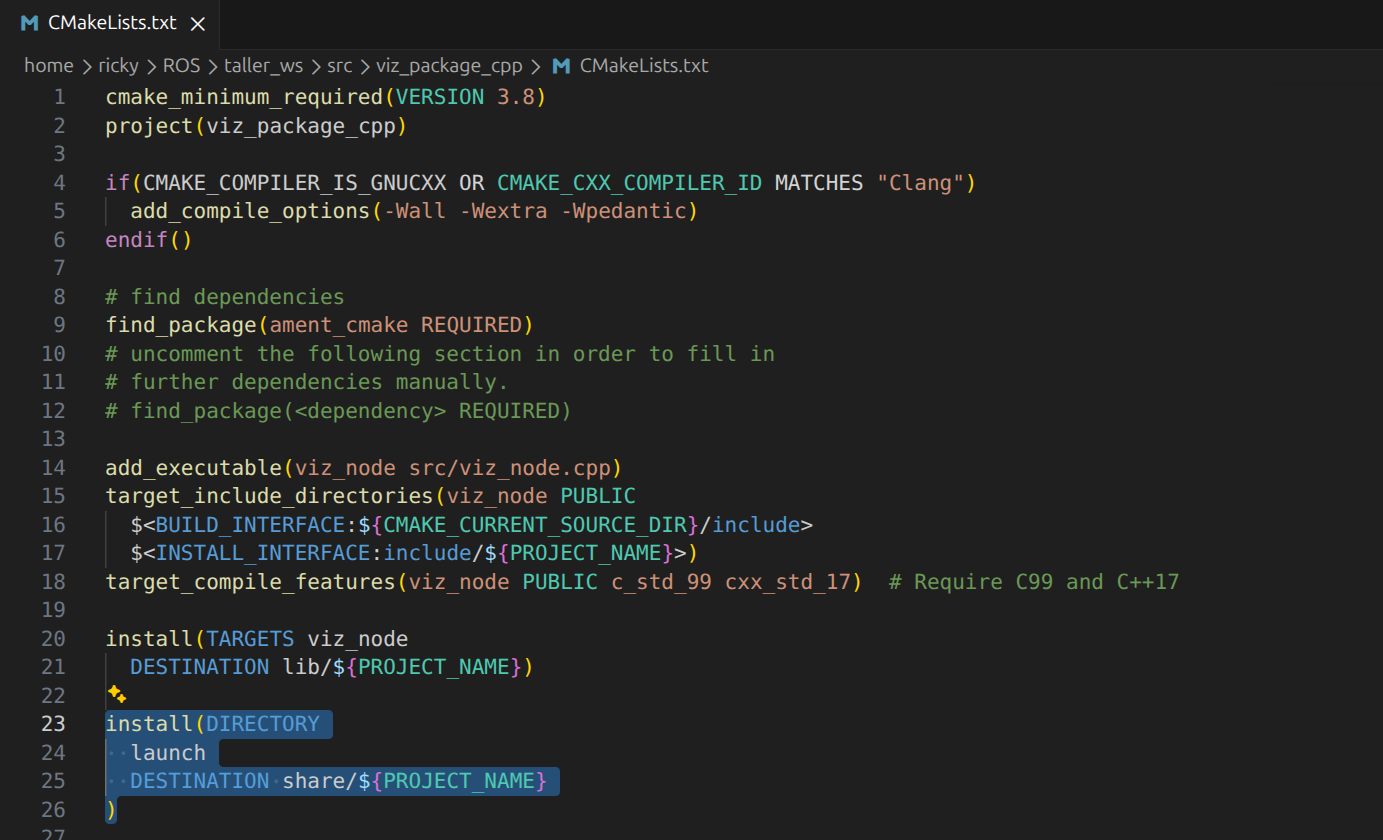
\includegraphics[width=1.4\textwidth]{imagenes/cmake.png}}
      \caption{Editar \texttt{CMakeLists.txt} para que los archivos launch se guarden en la carpeta \texttt{share}.}
      \label{fig:mi_imagen}
  \end{figure}
  
  \item En una terminal y en el espacio de trabajo, compilar con \texttt{colcon build}.
  \item En otra terminal y en el espacio de trabajo, activar el overlay con \texttt{source install/local\_setup.bash} y lanzar el launch file con \texttt{ros2 launch viz\_package\_cpp viz\_launch.py}
  
  \begin{figure}[H] 
      \centering    
      \makebox[\textwidth][c]{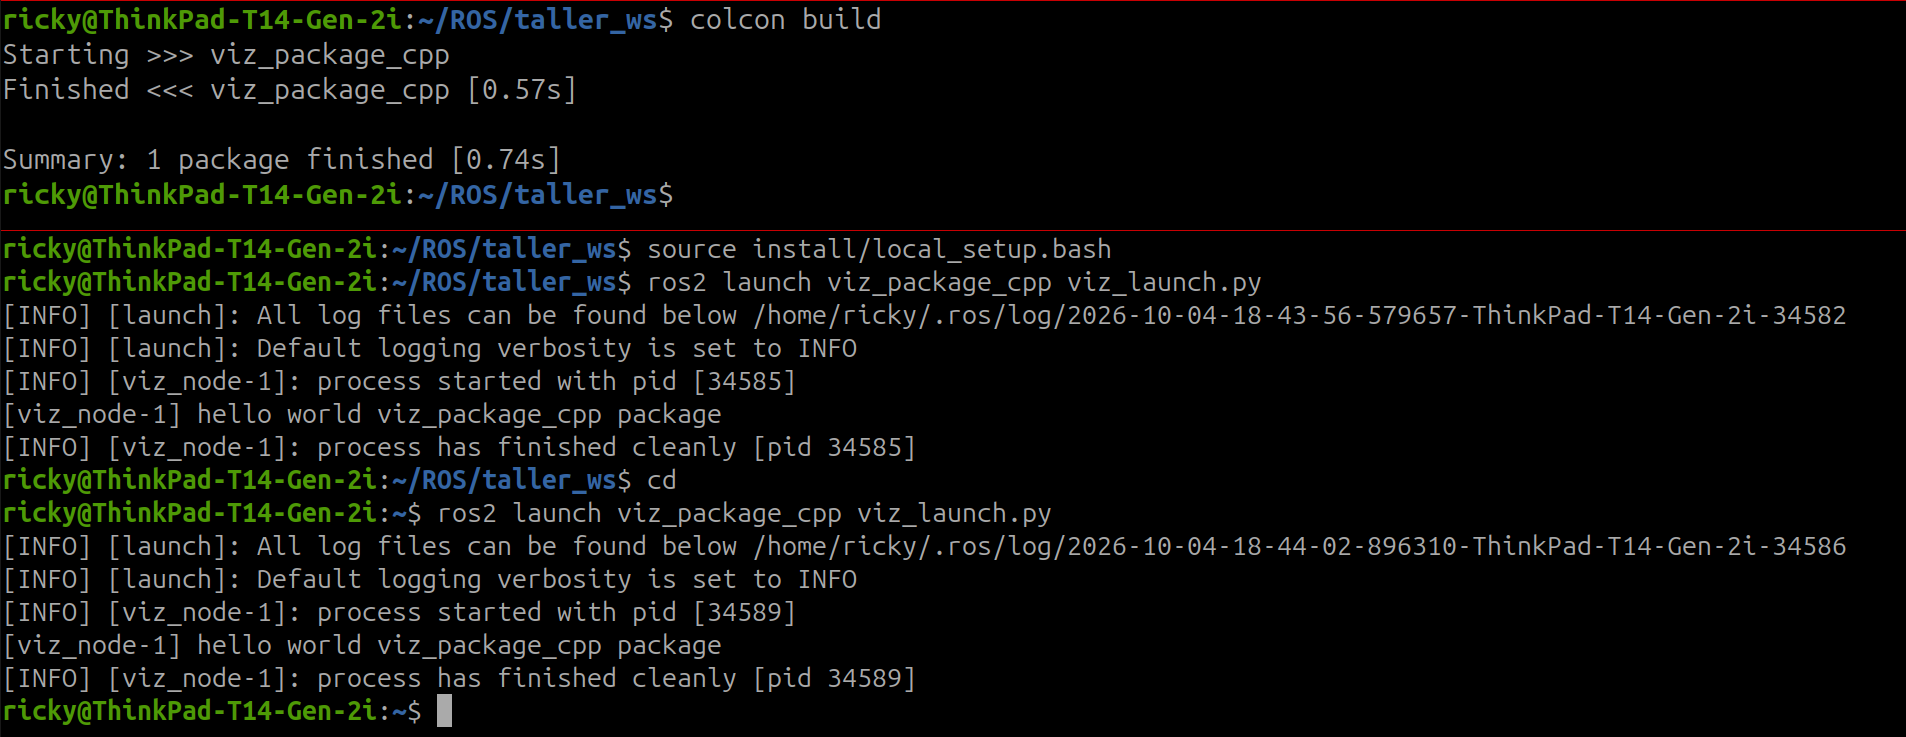
\includegraphics[width=1.4\textwidth]{imagenes/launchfinal.png}}
      \caption{Ahora se puede lanzar el launch file en cualquier ruta.}
      \label{fig:mi_imagen}
  \end{figure}

\end{enumerate}



\section{Modelado de Robots}
Ahora veremos cómo podemos construir y ver una visualización de un objeto en el programa rviz. Con eso, podremos construir una visualización de un robot.

Primero, creamos una carpeta llamada \texttt{urdf} dentro del paquete (justo debajo del paquete). Acá corregir, porque la imagen muestra que puse la carpeta en el espacio de trabajo y no en el paquete.

\begin{figure}[H] 
    \centering    
    \makebox[\textwidth][c]{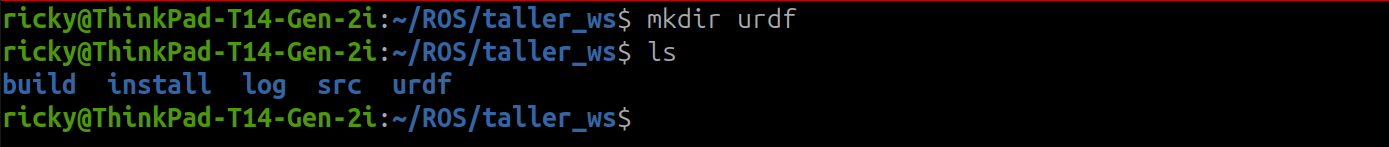
\includegraphics[width=1.4\textwidth]{imagenes/creacion-urdf.png}}
    \caption{Creación de carpeta urdf dentro del paquete.}
    \label{fig:mi_imagen}
\end{figure}

Ahora, vamos a crear un archivo \texttt{robot.urdf} dentro de la carpeta \texttt{urdf/}. \texttt{robot.urdf} contendrá lo siguiente:

\begin{center}
    \begin{Verbatim}[gobble=4]
    <?xml version="1.0"?>
    <robot name="paquito">
        <link name="base_link">
            <visual>
                <geometry>
                    <cylinder length="0.6" radius="0.2"/>
                </geometry>
                <material name="blue"><color rgba="0 0 .8 1"/></material>
            </visual>

            <collision>
                <geometry>
                    <cylinder length="0.6" radius="0.2"/>
                </geometry>
            </collision>
        </link>
    </robot>
    \end{Verbatim}
\end{center}

\begin{figure}[H] 
    \centering    
    \makebox[\textwidth][c]{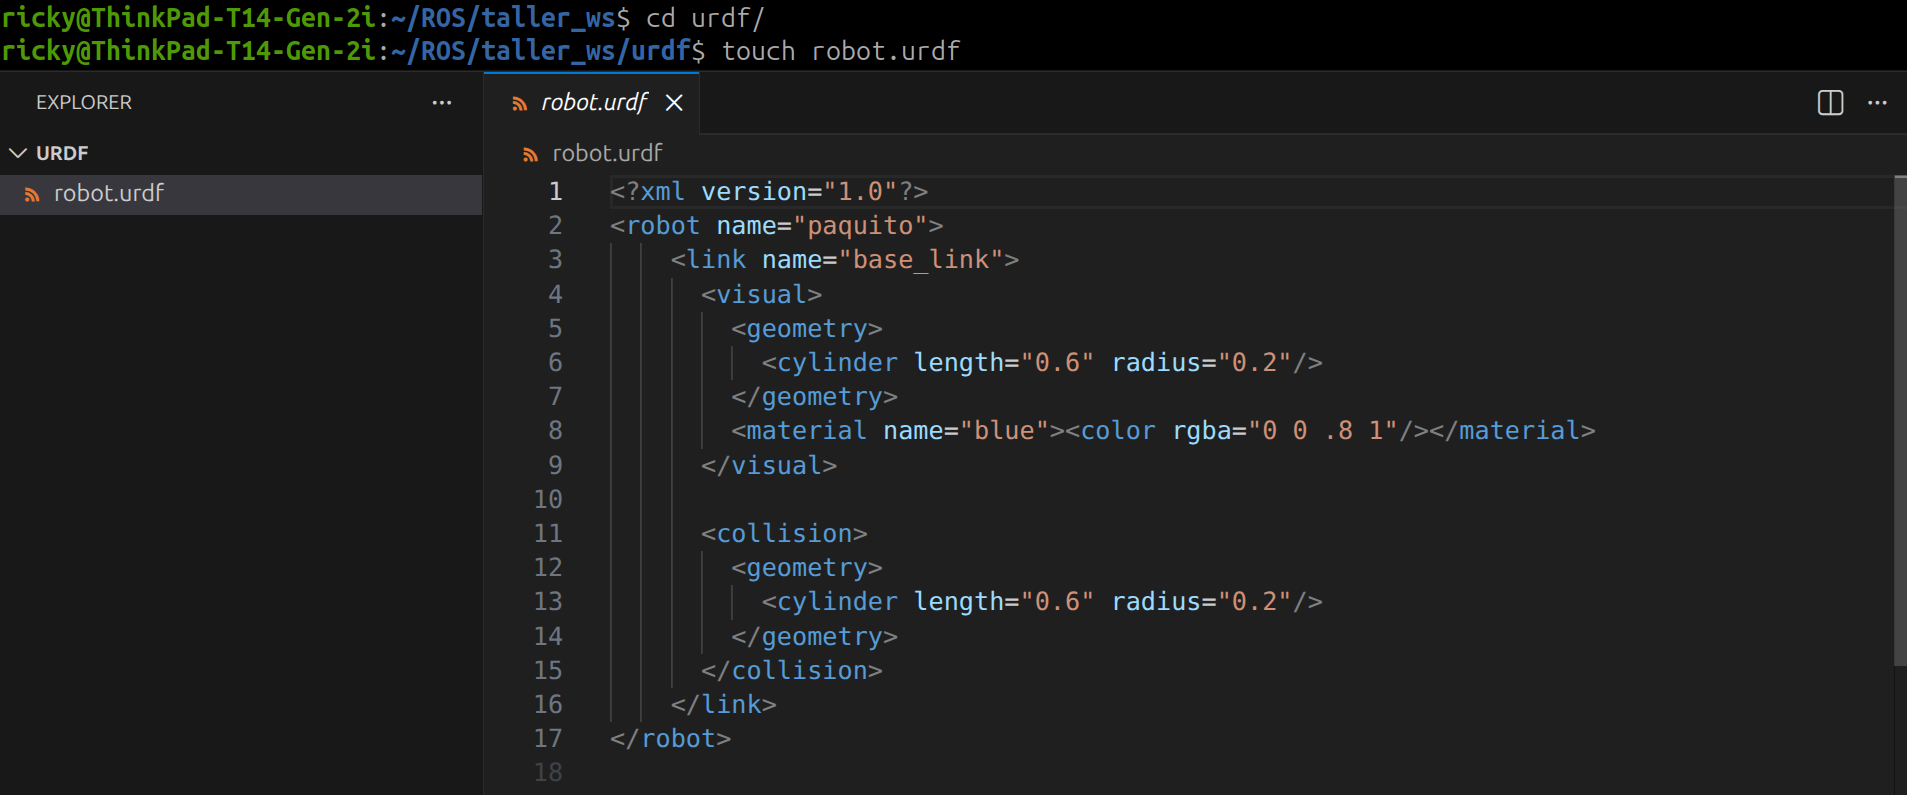
\includegraphics[width=1.4\textwidth]{imagenes/urdf2-3.png}}
    \caption{Creación de archivo robot.urdf.}
    \label{fig:mi_imagen}
\end{figure}

Luego, modificamos la línea \texttt{urdf} a la directiva install en el archivo \texttt{CMakeLists.txt}. La directiva install debe quedar como sigue:

\begin{center}
    \begin{Verbatim}[gobble=4]
        install (DIRECTORY
        launch 
        urdf # nueva línea
        DESTINATION share/${PROJECT_NAME}
        )
    \end{Verbatim}
\end{center}

\begin{figure}[H] 
    \centering    
    \makebox[\textwidth][c]{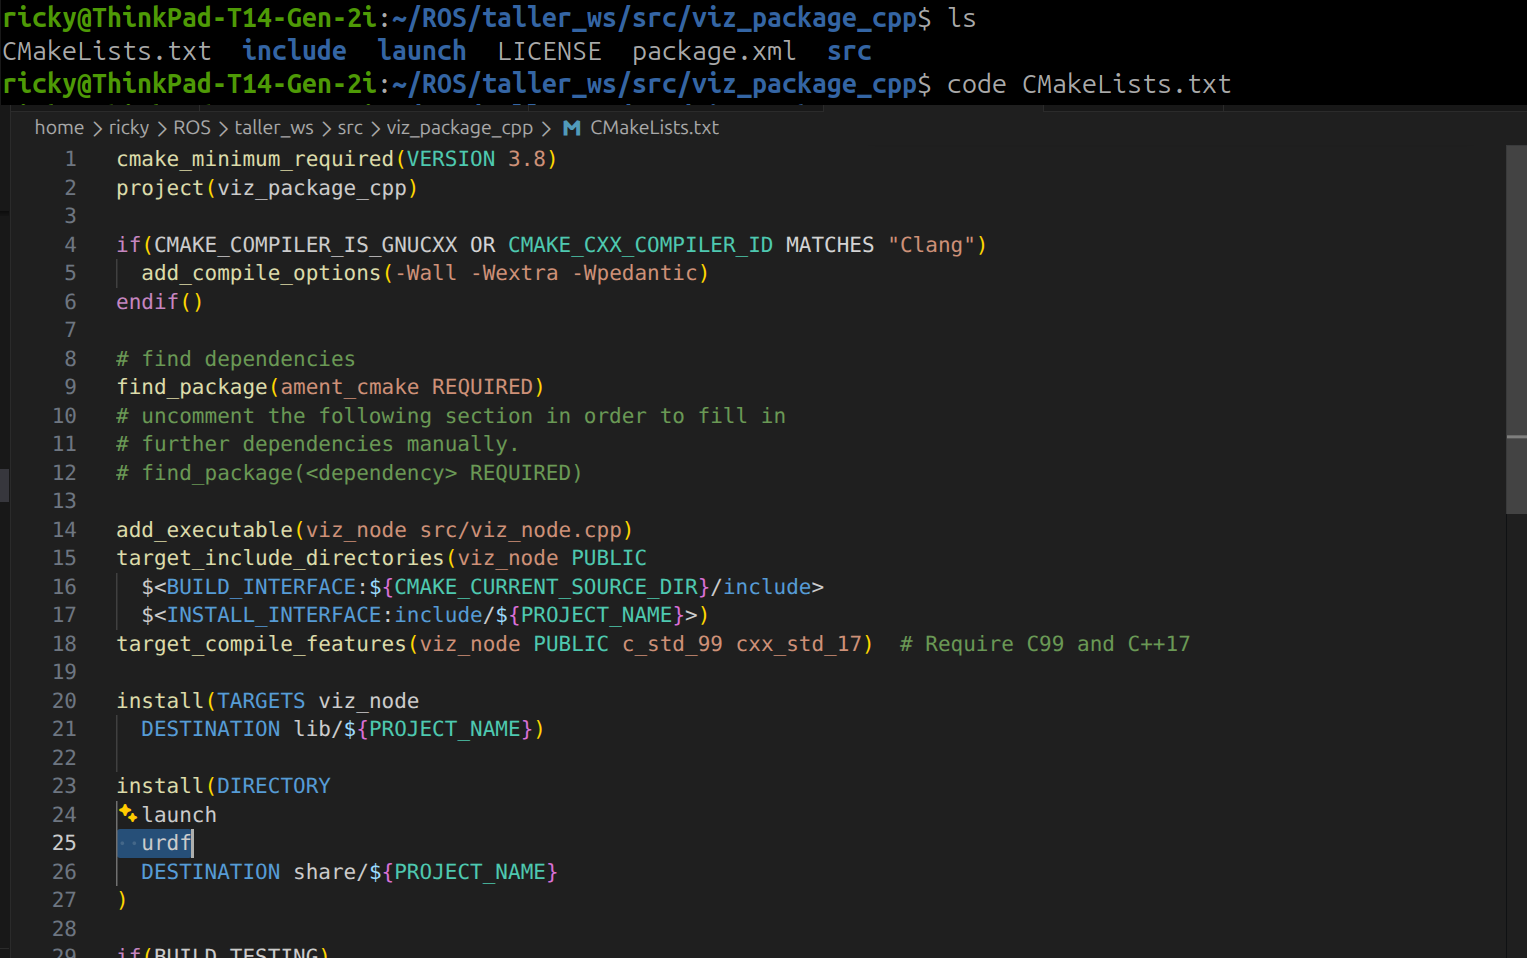
\includegraphics[width=1.4\textwidth]{imagenes/cmake-urdf3.png}}
    \caption{Agregar urdf a la directiva install del CMakeLists.txt.}
    \label{fig:mi_imagen}
\end{figure}

Ahora que ya tenemos la descripción de la forma del objeto a visualizar, pasaremos a la parte del movimiento. En el archivo \texttt{package.xml} del paquete, agregamos las siguientes líneas:

\begin{center}
    \begin{Verbatim}[gobble=4]
        <exec_depend>joint_state_publisher</exec_depend>
        <exec_depend>robot_state_publisher</exec_depend>
    \end{Verbatim}
\end{center}

\begin{figure}[H] 
    \centering    
    \makebox[\textwidth][c]{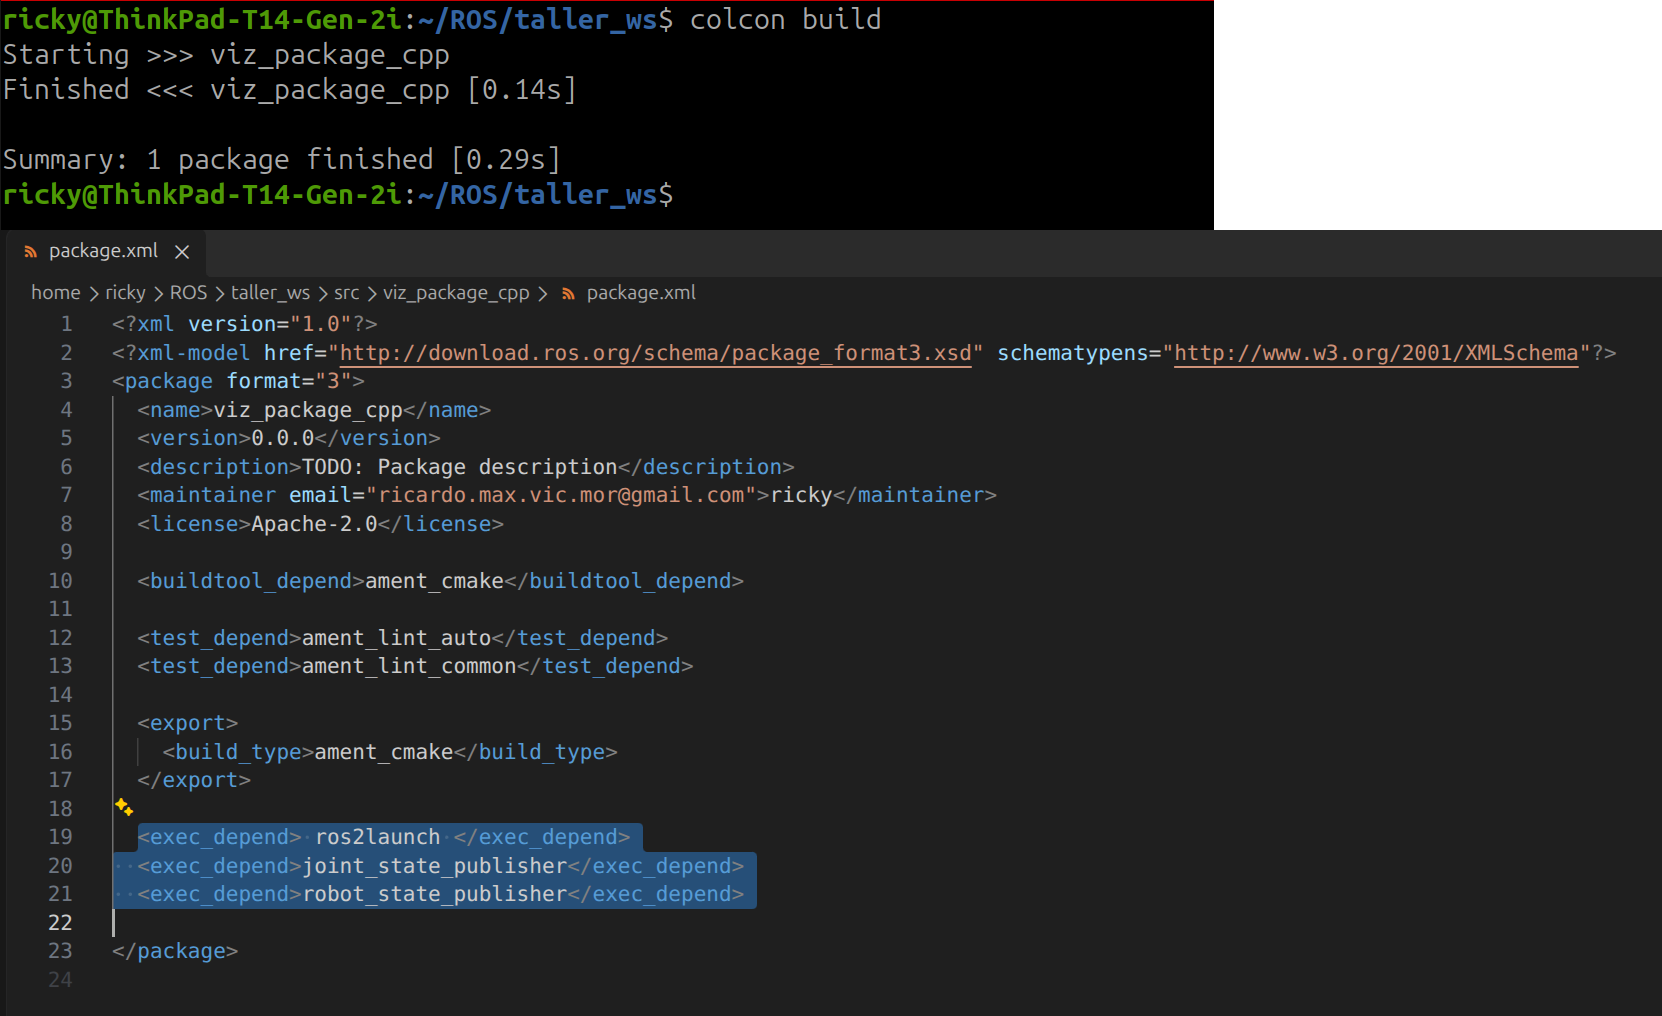
\includegraphics[width=1.4\textwidth]{imagenes/cmake52.png}}
    \caption{Modificación package.xml.}
    \label{fig:mi_imagen}
\end{figure}

Ejecutar el siguiente comando en el espacio de trabajo:

\begin{center}
    \begin{Verbatim}[gobble=4]
        rosdep install -i --from-path src --rosdistro jazzy -y        
    \end{Verbatim}
\end{center}

Si pide inicializar, ejecutar los comandos siguientes antes de ejecutar el comando anterior:

\begin{center}
    \begin{Verbatim}[gobble=4]
        sudo rosdep init
        rosdep update
    \end{Verbatim}
\end{center}


\begin{figure}[H] 
    \centering    
    \makebox[\textwidth][c]{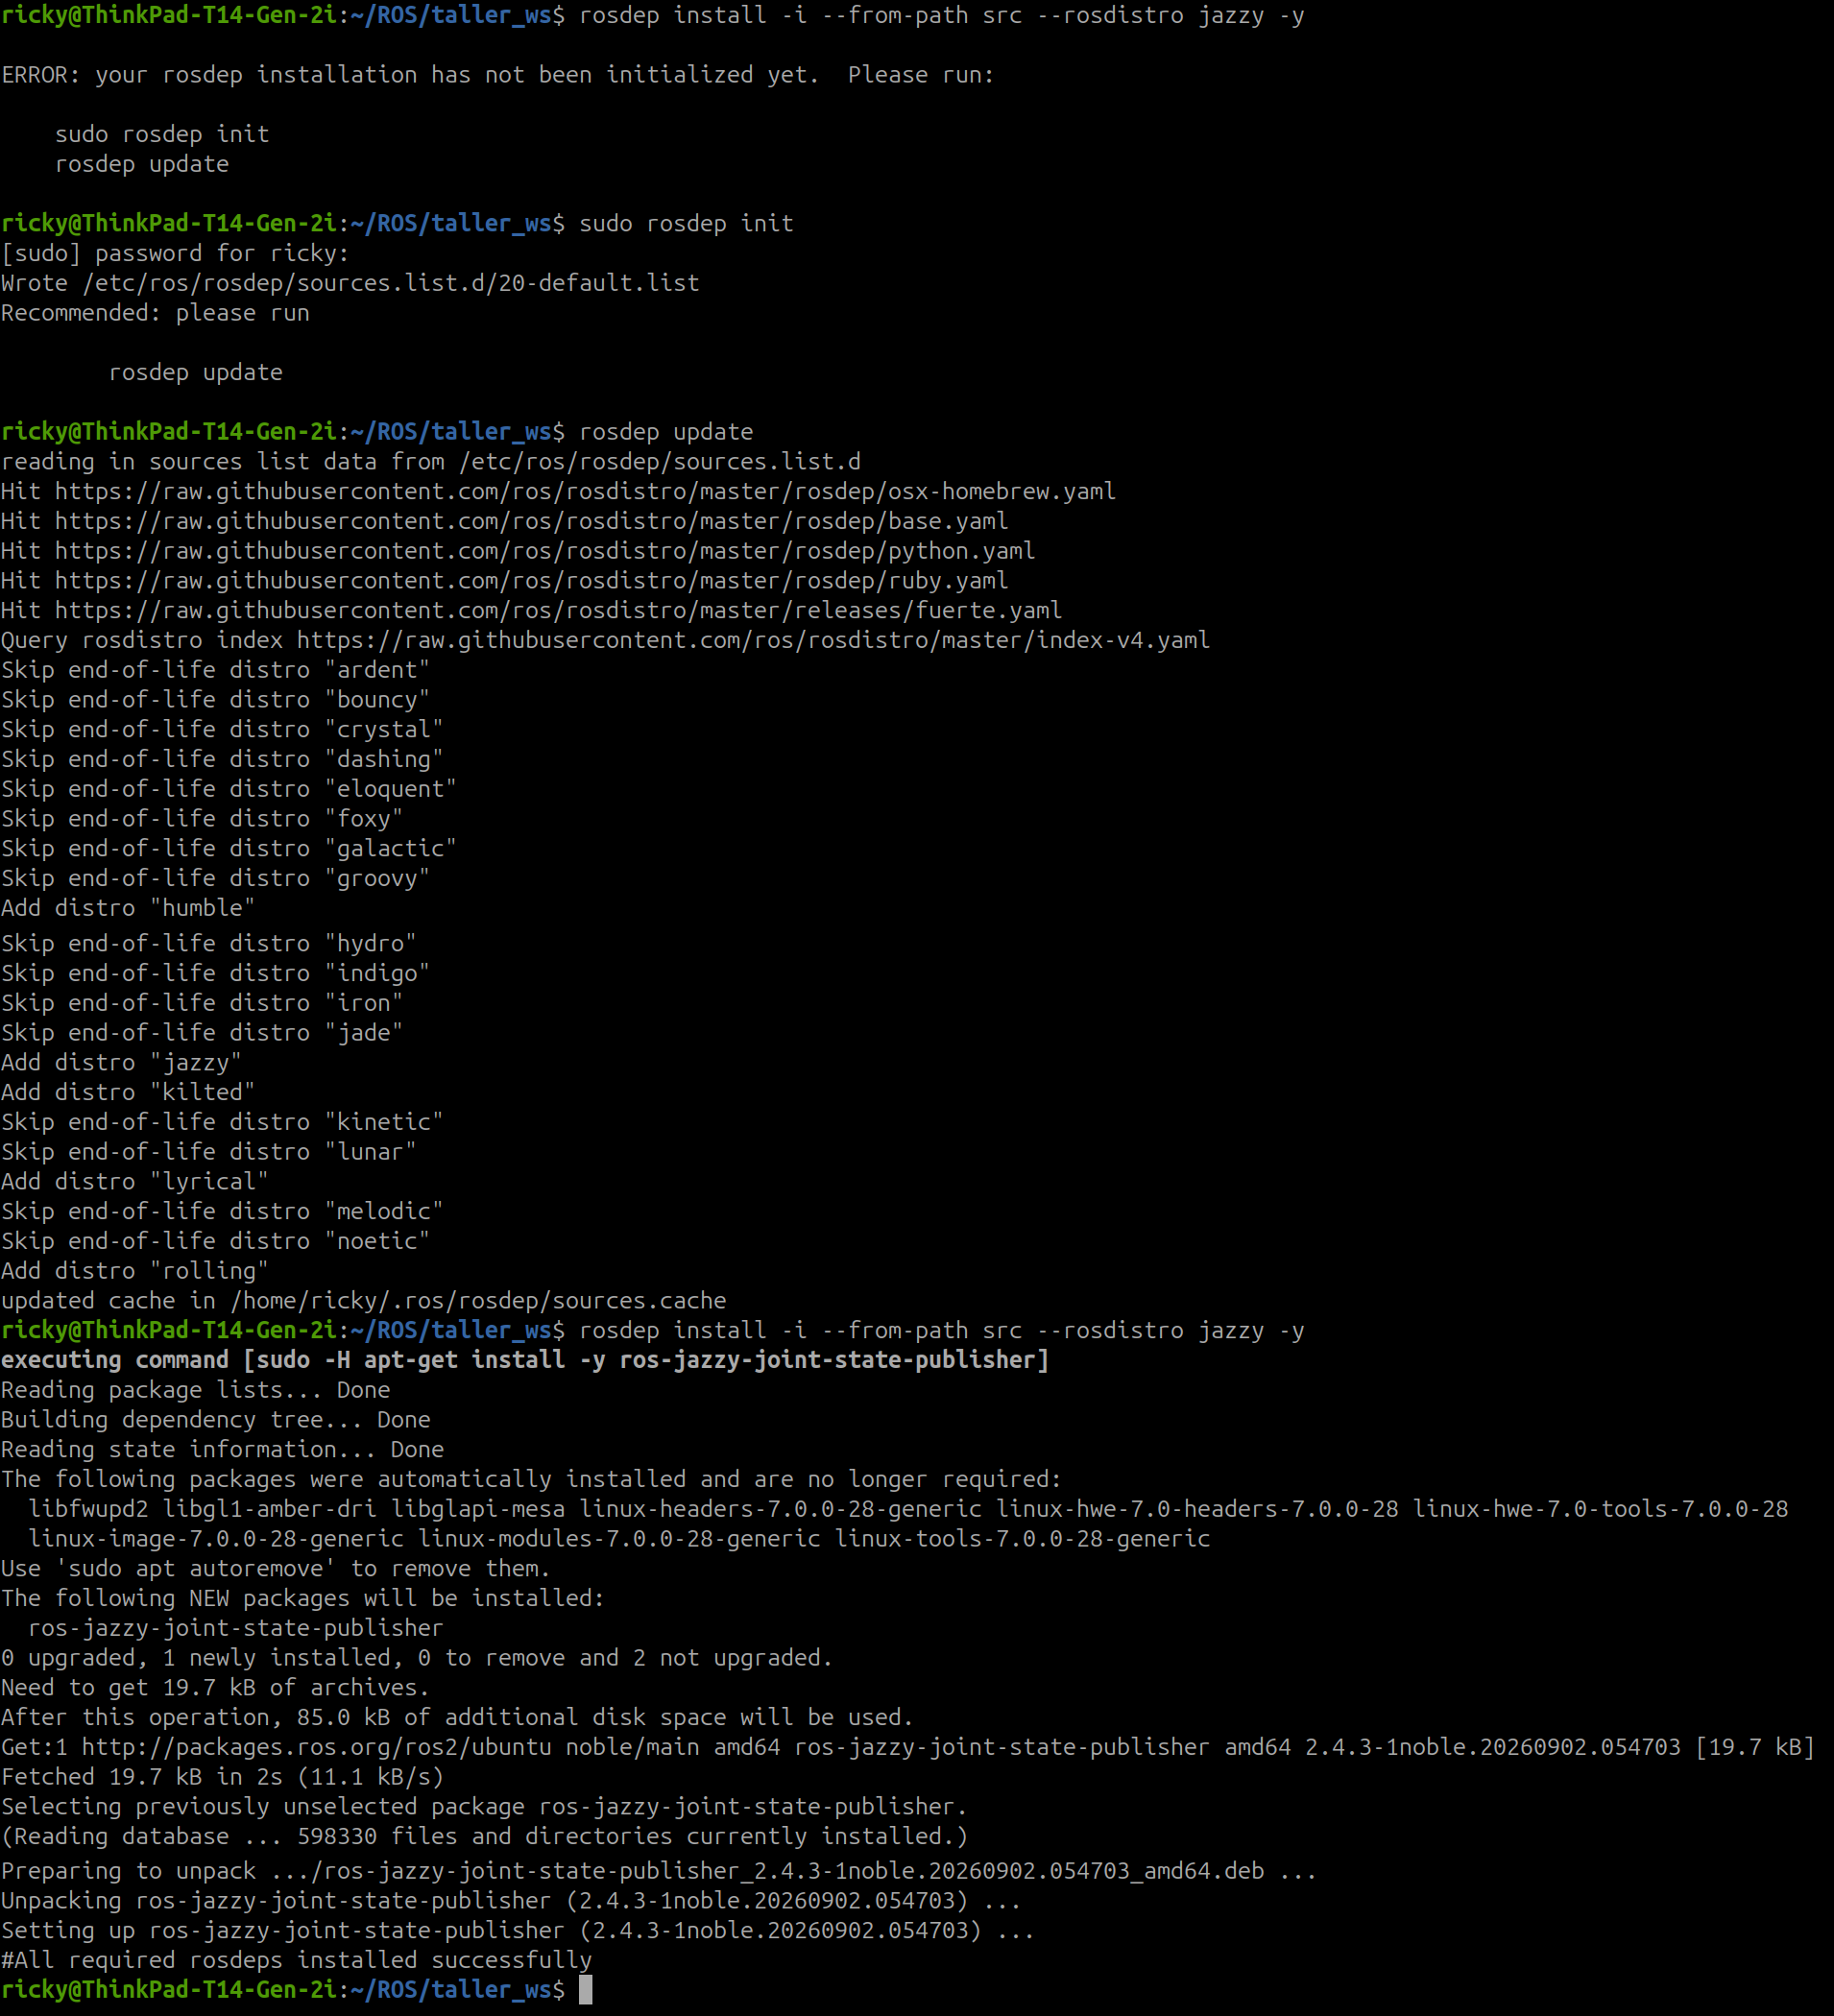
\includegraphics[width=1.4\textwidth]{imagenes/r123.png}}
    \caption{Instalación con rosdep.}
    \label{fig:mi_imagen}
\end{figure}

Ahora, hay que pedir al archivo de lanzamiento que ejecute al nodo que publicará la
descripción del robot. Modificamos al archivo \texttt{viz\_launch.py} para que quede de la siguiente forma.

\begin{center}
    \begin{Verbatim}[gobble=4]
        import os
        from ament_index_python.packages import get_package_share_directory
        from launch import LaunchDescription
        from launch_ros.actions import Node        
        
        def generate_launch_description():
        package_dir = get_package_share_directory('viz_package_cpp')
        path_to_urdf = os.path.join(package_dir, 'urdf', 'robot.urdf')
        
        with open(path_to_urdf, 'r') as f:
        robot_desc = f.read()
        
        return LaunchDescription([
            Node(
                package='viz_package_cpp',
                namespace='paquito1',
                executable='viz_node',
                name='viz',
                output='screen',
                ),
                Node(
                    package='robot_state_publisher',
                    name='robot_state_publisher',
                    executable='robot_state_publisher',
                    output='screen',
                    parameters=[{
                        'robot_description': robot_desc,
                        'publish_frequency': 30.0,
                        }]
                        )
                        ])
                        
                    \end{Verbatim}
                \end{center}
                
                
\begin{figure}[H] 
    \centering    
    \makebox[\textwidth][c]{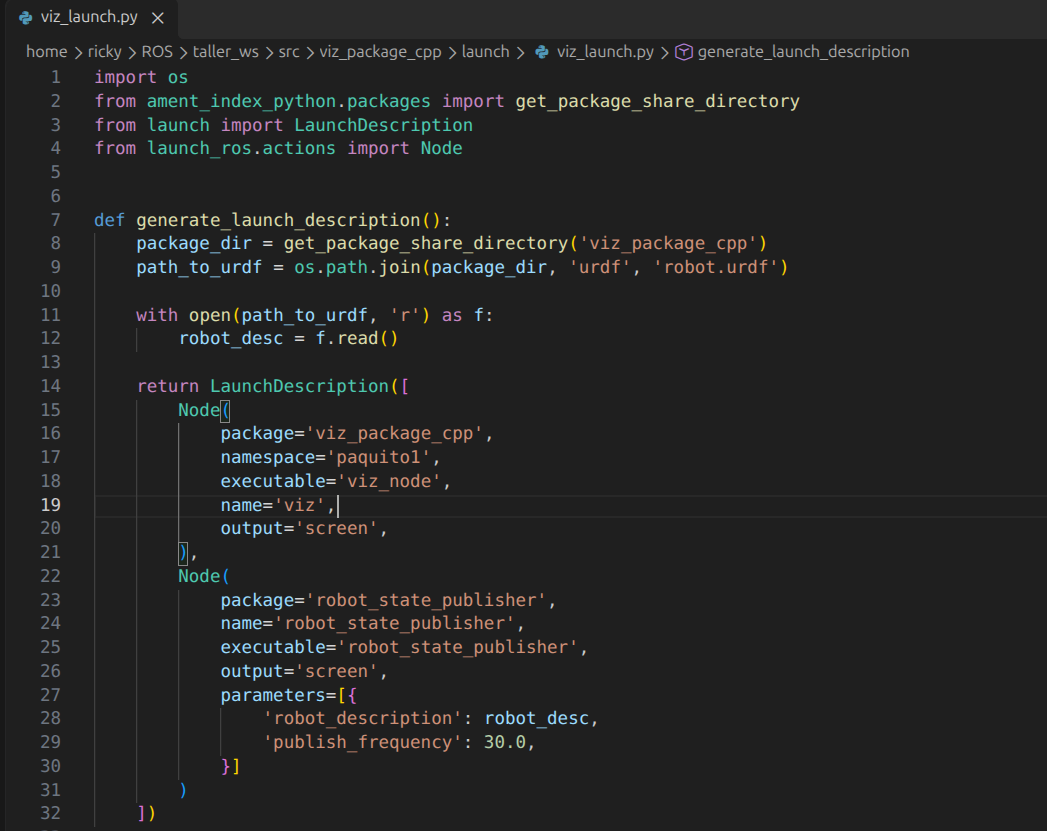
\includegraphics[width=1.4\textwidth]{imagenes/l2.png}}
    \caption{Modificación al launch file para publicar la figura.}
    \label{fig:mi_imagen}
\end{figure}
                
Ahora procedemos a compilar y lanzar el launchfile. Recordemos que esto se hace con los siguientes comandos y como sigue:                
                
\begin{center}
    \begin{Verbatim}[gobble=4]
    colcon build
    ros2 launch viz_package_cpp viz_launch.py
    \end{Verbatim}
\end{center}

\begin{figure}[H] 
    \centering    
    \makebox[\textwidth][c]{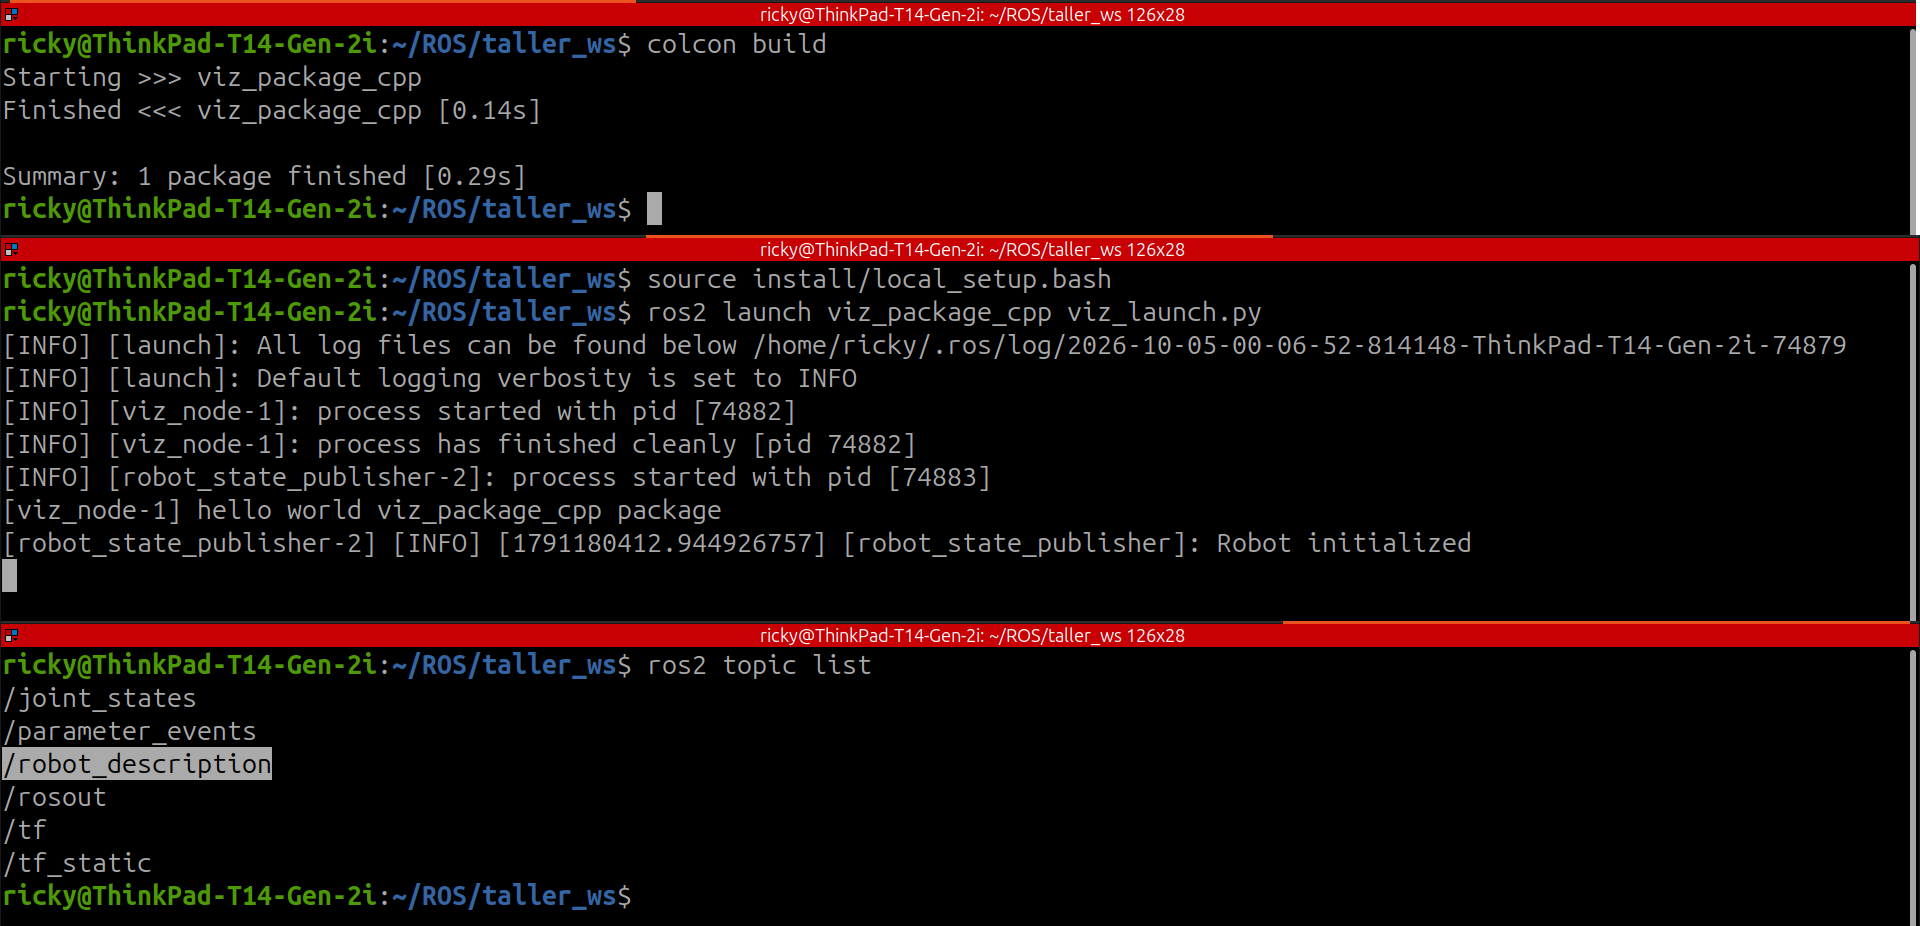
\includegraphics[width=1.4\textwidth]{imagenes/rdesc123.png}}
    \caption{Compilación, lanzamiento de launch file y listado de tópicos.}
    \label{fig:mi_imagen}
\end{figure}

Vemos de la figura anterior, en la terminal 2, que se sigue ejecutando el nodo de hola mundo, y además se ejecuta el segundo nodo que publica la descripción del robot. Podemos comprobar que se publica la descripción del robot en la terminal 3, porque se publica el tópico \texttt{/robot\_description}.







\section{Rviz}
Continuaremos con lo anteriore. Veremos cómo podemos abrir el programa de visualización rviz utilizando el launch file.

Creamos una carpeta \texttt{rviz} al lado de la carpeta \texttt{urdf}. Luego abrimos rviz en terminal con el comando \texttt{rviz2}.

\begin{center}
    \begin{Verbatim}[gobble=4]
    rviz2
    \end{Verbatim}
\end{center}

Dentro de rviz, en el menú superior, en file, seleccionar Save Config As, como se muestra en la siguiente imagen:

\begin{figure}[H] 
    \centering    
    \makebox[\textwidth][c]{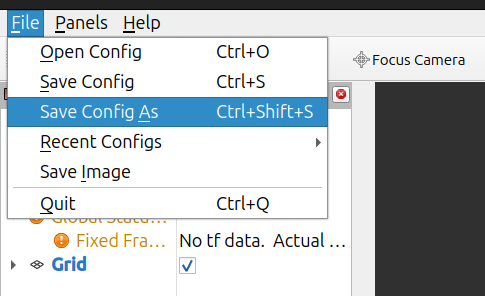
\includegraphics[width=1.4\textwidth]{imagenes/file-save-config.png}}
    \caption{rviz2, file, save config as.}
    \label{fig:mi_imagen}
\end{figure}

luego nombrar al archivo como panel.rviz, y guardar ese archivo en la carpeta \texttt{rviz} que acabamos de crear, como se muestra en la siguiente imagen:

\begin{figure}[H] 
    \centering    
    \makebox[\textwidth][c]{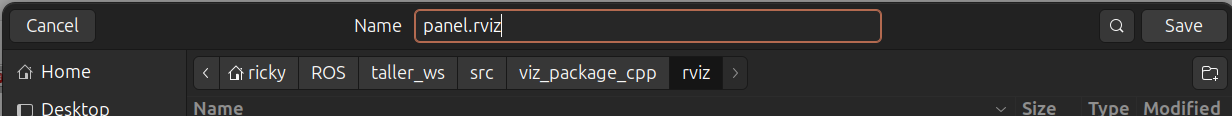
\includegraphics[width=1.4\textwidth]{imagenes/save-config2.png}}
    \caption{Guardamos archivo panel.rviz en la carpeta rviz.}
    \label{fig:mi_imagen}
\end{figure}

Ahora vamos a agregar esta nueva carpeta \texttt{rviz} al install del archivo CMakeLists.txt, como se muestra en la siguiente imagen.

\begin{figure}[H]
    \centering
    \makebox[\textwidth][c]{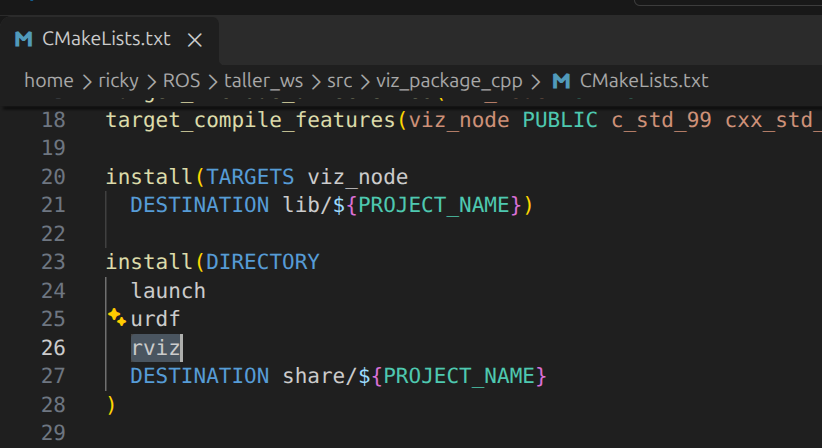
\includegraphics[width=1.4\textwidth]{imagenes/install-rviz-cmake.png}}
    \caption{Agregamos rviz al install del CMakeLists.txt}
    \label{fig:mi_imagen}
\end{figure}

Luego, agregamos un nuevo nodo en el launch file del paquete, este nodo abrirá rviz2 cuando se ejecute. Modificamos el launch file como se ve en la siguiente imagen:

\begin{figure}[H]
    \centering
    \makebox[\textwidth][c]{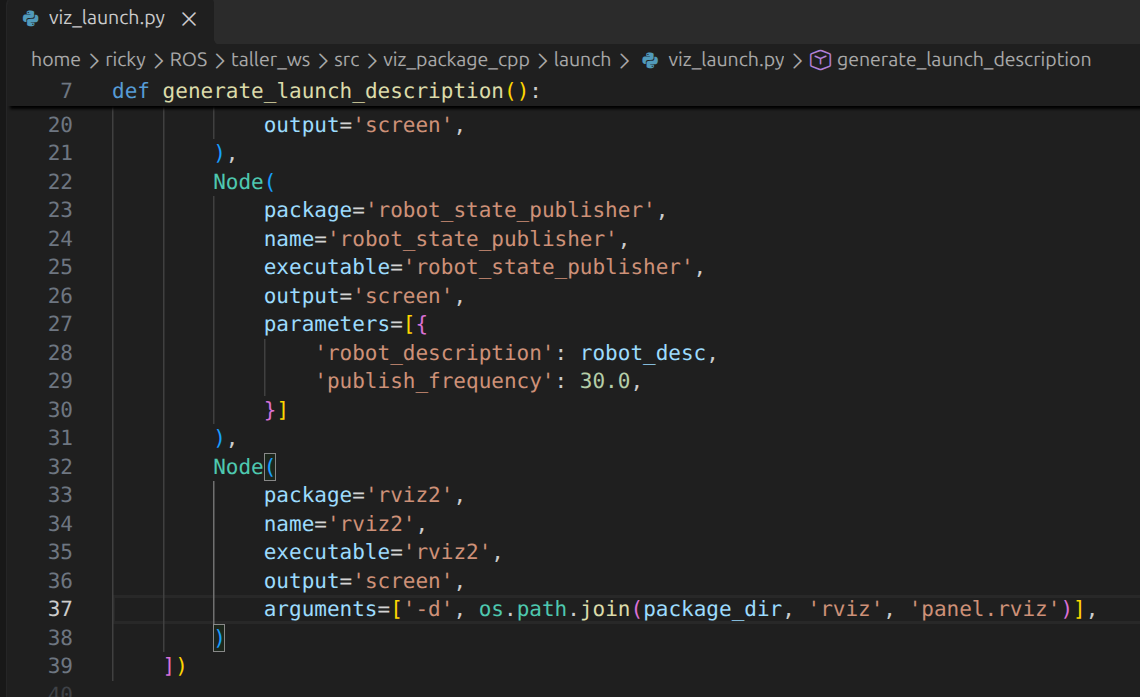
\includegraphics[width=1.4\textwidth]{imagenes/launch-rviz.png}}
    \caption{}
    \label{fig:mi_imagen}
\end{figure}

Ahora, en la terminal 1 compilamos con \texttt{colcon build}, en la terminal 2 lanzamos el launch file con \texttt{ros2 launch viz\_package\_cpp viz\_launch.py}. Esto se muestra en las siguientes imagenes:

\begin{figure}[H]
    \centering
    \makebox[\textwidth][c]{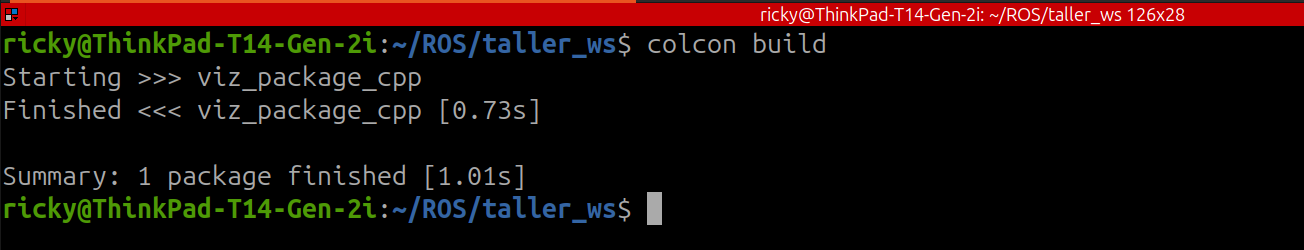
\includegraphics[width=1.4\textwidth]{imagenes/1:3-1.png}}
    \caption{}
    \label{fig:mi_imagen}
\end{figure}

\begin{figure}[H]
    \centering
    \makebox[\textwidth][c]{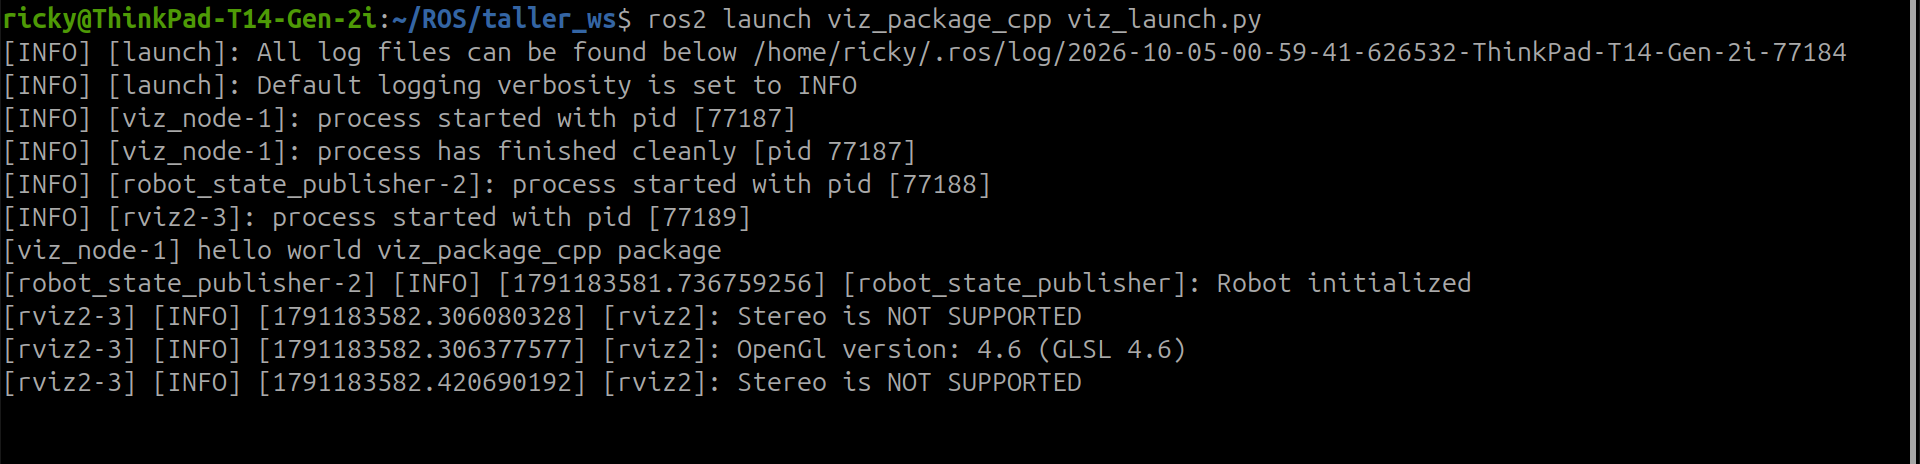
\includegraphics[width=1.4\textwidth]{imagenes/1:3-2.png}}
    \caption{}
    \label{fig:mi_imagen}
\end{figure}

\begin{figure}[H]
    \centering
    \makebox[\textwidth][c]{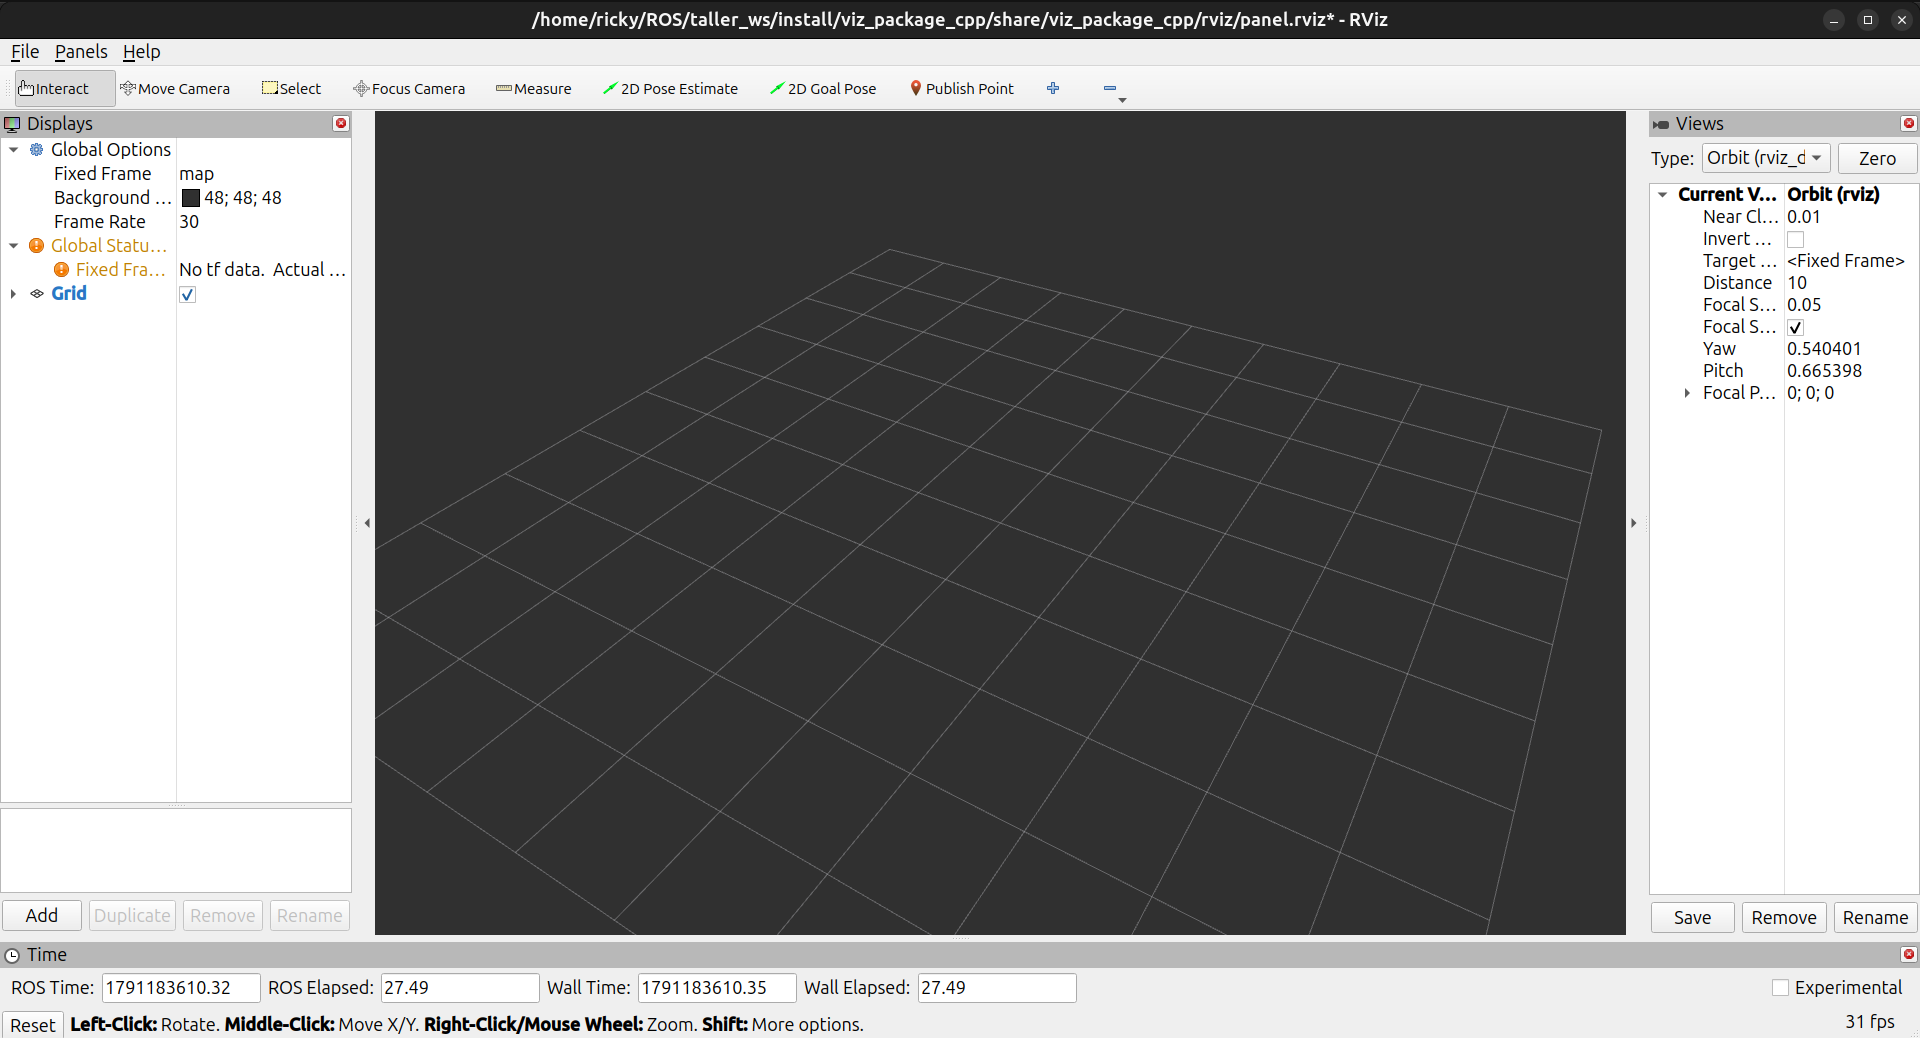
\includegraphics[width=1.4\textwidth]{imagenes/1:3-3.png}}
    \caption{}
    \label{fig:mi_imagen}
\end{figure}

Ahora, con el rviz abierto, en el menú de la izquierda, en la parte que dice Displays, seleccionamos el campo a la derecha de donde dice Fixed Frame, y cambiamos lo que dice map a base\_link. Esto se muestra en las siguientes imágenes:

\begin{figure}[H]
    \centering
    \makebox[\textwidth][c]{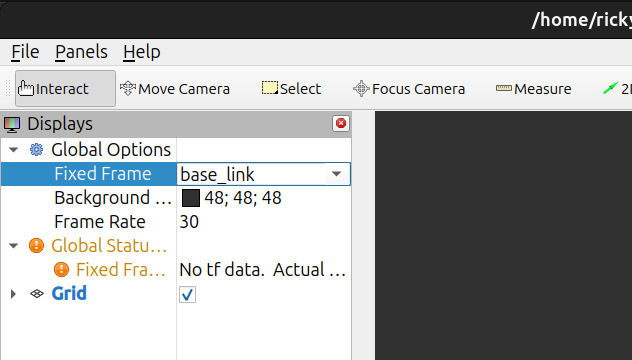
\includegraphics[width=1.4\textwidth]{imagenes/ffbl.png}}
    \caption{}
    \label{fig:mi_imagen}
\end{figure}

Ahora, en rviz, seleccionamos el boton que dice Add (que está abajo a la izquierda), y en la pestaña que dice By Display Type, seleccionamos RobotModel. Como se ve en la siguiente imagen:

\begin{figure}[H]
    \centering
    \makebox[\textwidth][c]{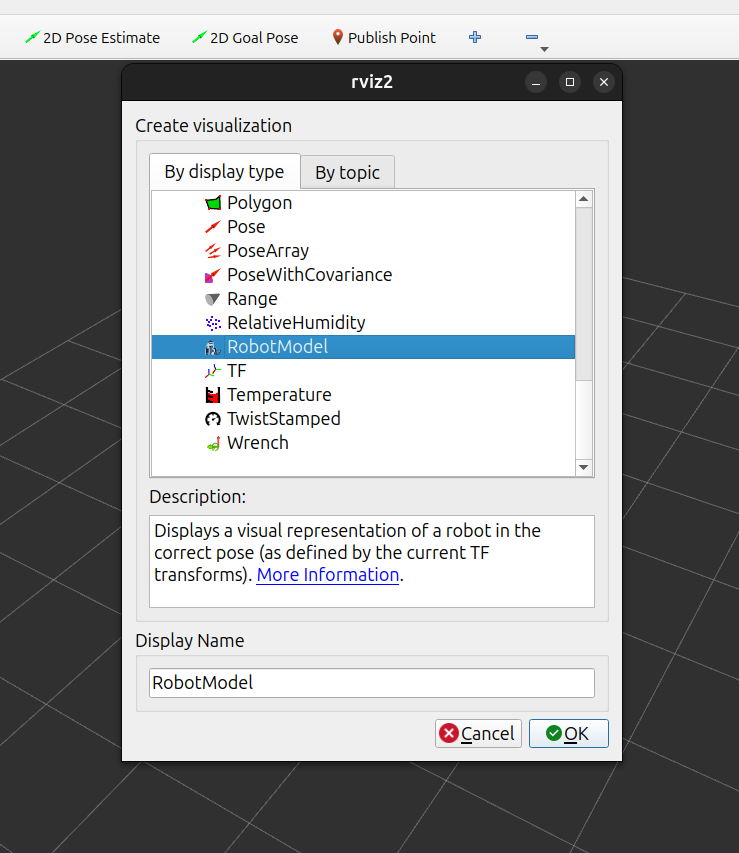
\includegraphics[width=1.4\textwidth]{imagenes/rmodel.png}}
    \caption{}
    \label{fig:mi_imagen}
\end{figure}

Ahora, en el menu de la izquierda aparecerá en un nuevo apartado que dice RobotModel, y en la opción Description topic, seleccionamos la opción que dice /robot\_description. Como se muestra en la imagen siguiente:

\begin{figure}[H]
    \centering
    \makebox[\textwidth][c]{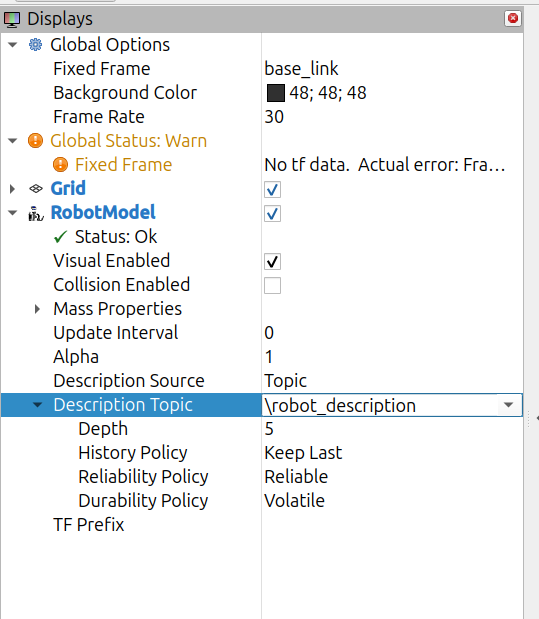
\includegraphics[width=1.4\textwidth]{imagenes/rdescriptionrviz.png}}
    \caption{}
    \label{fig:mi_imagen}
\end{figure}


Con las configuraciones anteriores, se debería de mostrar la pieza (nuestro robot hasta ahora) que definimos anteriormente en el archivo .urdf. 

\begin{figure}[H]
    \centering
    \makebox[\textwidth][c]{\includegraphics[width=1.4\textwidth]{imagenes/pieza.png}}
    \caption{}
    \label{fig:mi_imagen}
\end{figure}



% Fin del documento
\end{document}
